\documentclass[border=5pt]{standalone}
\usepackage{tikz}
\usetikzlibrary{arrows.meta,calc,positioning}

\begin{document}
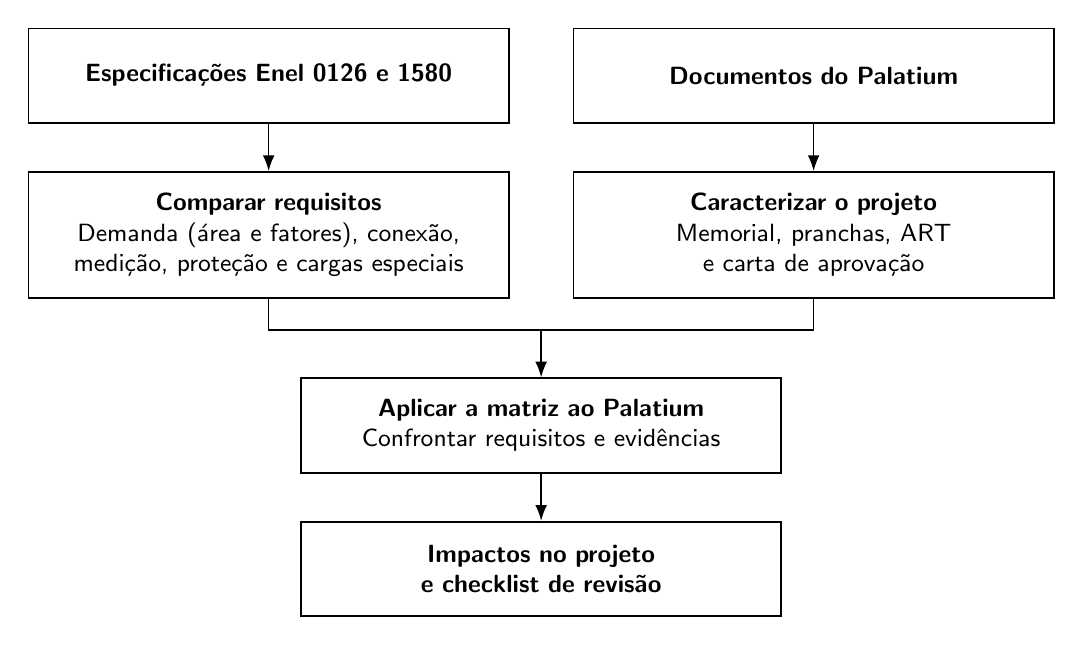
\begin{tikzpicture}[
  caixa/.style={
    draw=black,
    line width=0.6pt,
    text=black,
    align=center,
    minimum height=12mm,
    text width=57mm,
    inner sep=2mm,
    font=\sffamily\small
  },
  seta/.style={-{Latex[length=2mm,width=1.5mm]},line width=0.6pt,draw=black},
  linha/.style={line width=0.6pt,draw=black}
]
  \node[caixa] (normas) {\textbf{Especificações Enel 0126 e 1580}};
  \node[caixa,right=8mm of normas] (documentos) {\textbf{Documentos do Palatium}};

  \node[caixa,minimum height=16mm,below=6mm of normas] (comparacao) {
    \textbf{Comparar requisitos}\\
    Demanda (área e fatores), conexão,\\
    medição, proteção e cargas especiais
  };
  \node[caixa,minimum height=16mm,below=6mm of documentos] (caracterizacao) {
    \textbf{Caracterizar o projeto}\\
    Memorial, pranchas, ART e carta de aprovação
  };

  \coordinate (centro) at ($(comparacao.south)!0.5!(caracterizacao.south)$);
  \node[caixa,below=10mm of centro] (matriz) {
    \textbf{Aplicar a matriz ao Palatium}\\
    Confrontar requisitos e evidências
  };
  \node[caixa,below=6mm of matriz] (saida) {
    \textbf{Impactos no projeto e checklist de revisão}
  };

  \draw[seta] (normas) -- (comparacao);
  \draw[seta] (documentos) -- (caracterizacao);
  \coordinate[below=4mm of centro] (juncao);
  \draw[linha] (comparacao.south) |- (juncao) -| (caracterizacao.south);
  \draw[seta] (juncao) -- (matriz.north);
  \draw[seta] (matriz) -- (saida);
\end{tikzpicture}
\end{document}
